\documentclass{article}
\usepackage[utf8]{inputenc}
\usepackage[colorlinks, allcolors=blue]{hyperref}
\usepackage{graphicx}



\title{Remote Sensing and GIS Integration Portfolio}
\author{Robert Vlasakker, van de}
\date{June 2021}

% Location of the images
\graphicspath{{figures/}}


\begin{document}


\maketitle
\section{Introduction}
As I am a student from last year, I included one interactive map and one analogue map.
All code and output can be found on this \href{https://github.com/RobertvdV/GRS60312_RemoteSensingAndGISIntergration_IDV_Portfolio}{GitHub}.
As I do not own the data, the data for both maps is not provided.
For the interactive visualization I used a Folium map that I made for a master student Forest \& Nature Conservation. 
For the static map I made some new visualizations with data from the ACT course. 
These data contain LinearRings which I think are very interesting.

\section{Digital Visualization}
\textbf{Course Name \& Code.}
This interactive map was made for a master student that had trouble with Python Folium maps. 
So it has no specific course name and course code. 
It was for a master internship for the study Forest and Nature Conservation.
\\

\noindent
\textbf{Description of the Application.}
The interactive map contains the location of cows over time as a heat map. 
Each cow had a GNNS sensor that reports the location every hour.
This map now shows the location of all the cows every hour. 
The time interval is set quite high as the sensors cover about three weeks of information (so the total amount of timestamps will be the amount of hours in three weeks.
\\

\noindent
\textbf{Description \& Requirements of Users.}
The potential users of the map were the master student and the viewers of the student's presentation.
The maps was used for a presentation to see how the cows moved through the park over time.
The watcher of the presentation were mostly managers of the park. 
This was a initial map to check to cows location. 
The main goal of the master internship was to locate high risk areas of the park.
A high risk area was defined as an area where cows and recreational users of the park were close.
\\

\noindent
\textbf{Purpose of your visualization.}
The purpose of the interactive map was to see how the cows moved over time through the park to get an initial idea where the cows were.
\\

\noindent
\textbf{Motivation for choice of visualization type.}
As the data contained time series an interactive map was the best choice. 
\\

\noindent
\textbf{Data sets.}
The dataset was a csv file containing 15666 rows and 17 columns.
An example of a part of the data can be found in Figure \ref{fig:csvfile}.
\\

\begin{figure}[ht]
    \centering
    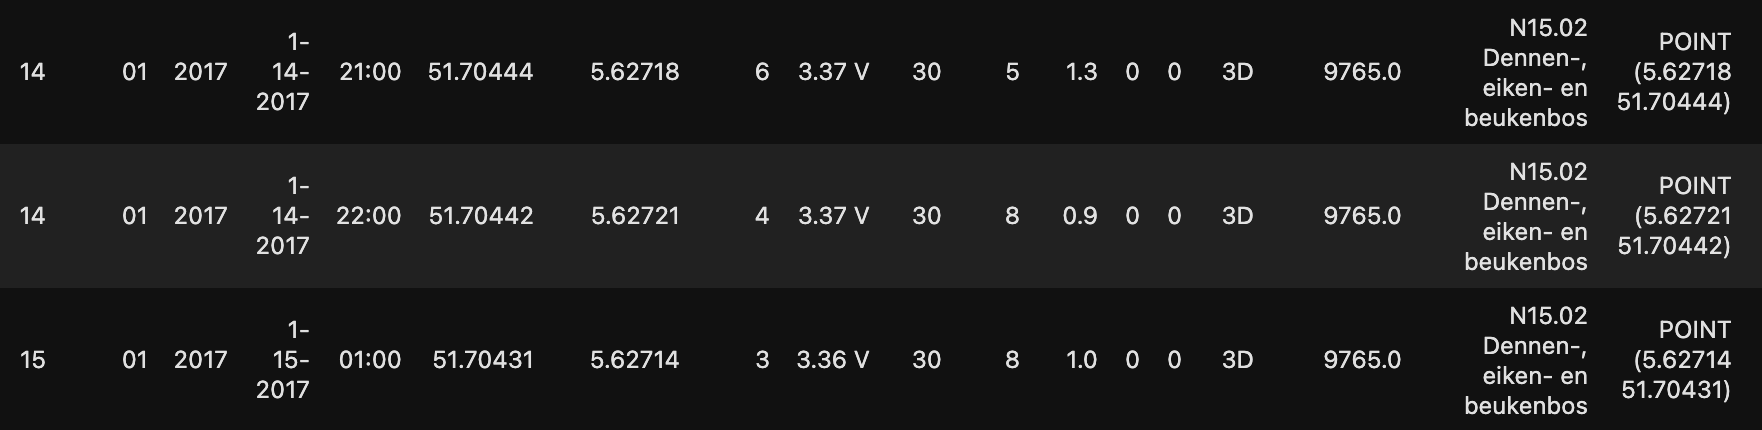
\includegraphics[width=\textwidth, height=\textheight, keepaspectratio]{csv.png}
    \caption{Example of the data}
    \label{fig:csvfile}
\end{figure}



\noindent
\textbf{Data Processing.}
The Folium map was made using Python and several libraries.
Pandas/GeoPandas was used to read the csv file to read the geometry and the attributes.
Several data transformation were made to make the data more redouble for the Folium package.
All the points had to be grouped by their cow ID, so all the cow ID of a single timestamp could be plotted on the map.
The Jupyter Notebook (data not provided) containing all the code (including the saving of the map) can be found via this \href{https://github.com/RobertvdV/GRS60312_RemoteSensingAndGISIntergration_IDV_Portfolio/blob/master/notebooks/1.0-TimeStampFoliumMap.ipynb}{link}.
\\

\noindent
\textbf{Implementation.}
The final result can be saved as an HMTL file. This file can be opened on any computer/tablet/phone that has a browser.
The final result can be downloaded via this \href{https://github.com/RobertvdV/GRS60312_RemoteSensingAndGISIntergration_IDV_Portfolio/blob/master/data/processed/HeathMapPerDag.html}{link} and an example of the final map can be found in Figure \ref{fig:finalmap}.
\\
\begin{figure}[ht]
    \centering
    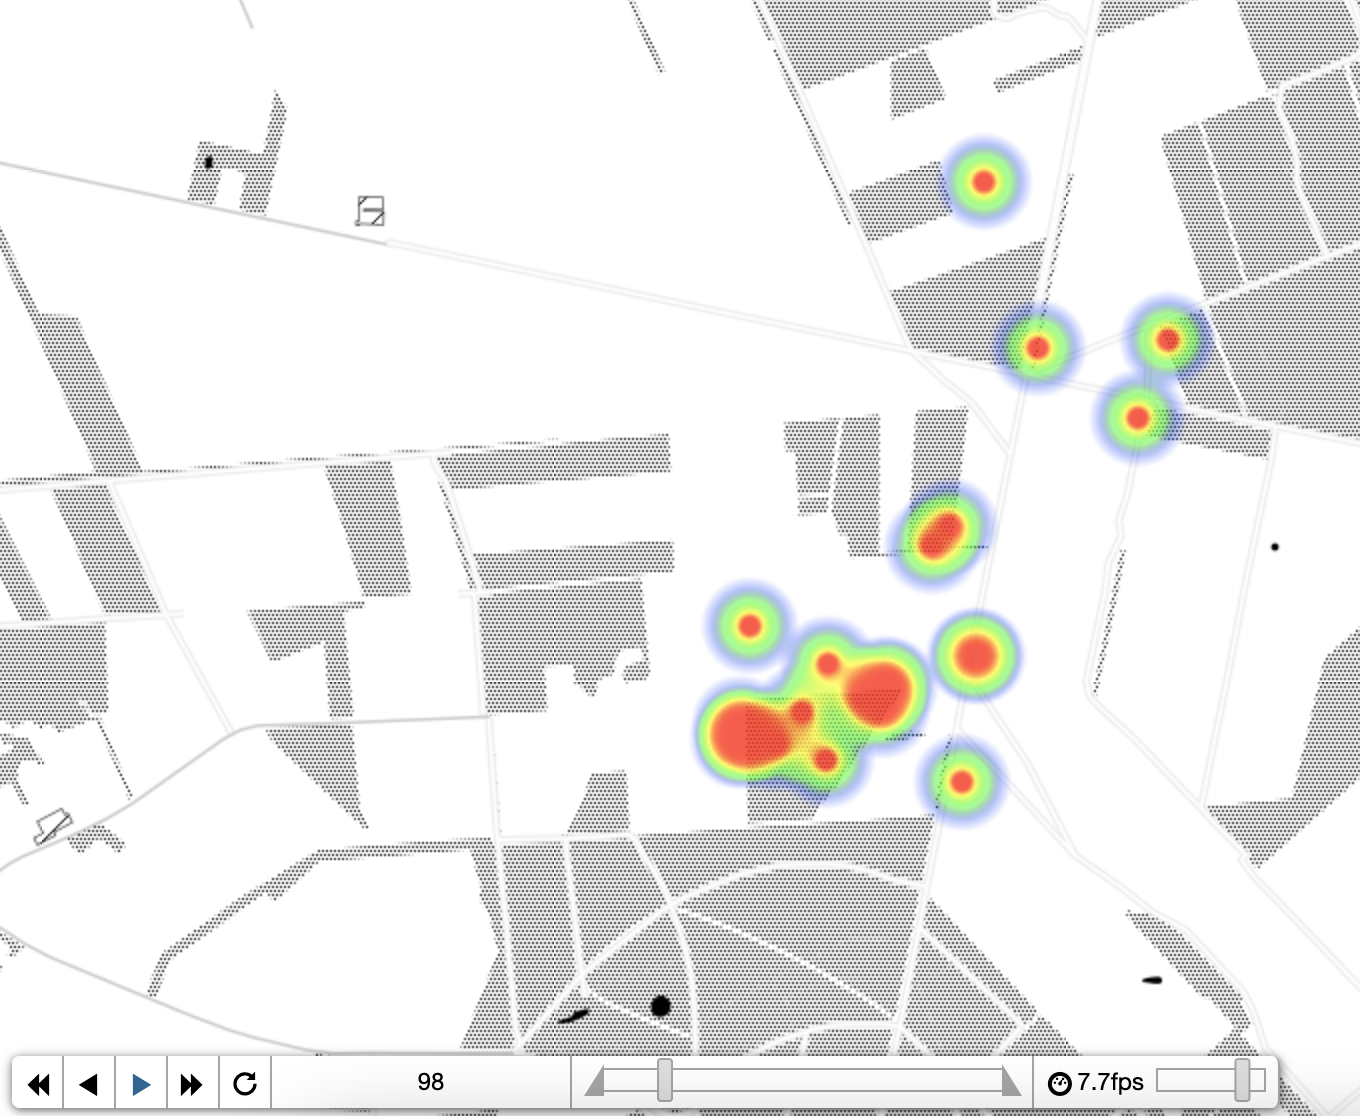
\includegraphics[width=\textwidth, height=\textheight, keepaspectratio]{finalmap.png}
    \caption{Example of the final map}
    \label{fig:finalmap}
\end{figure}

\noindent
\textbf{Reflection on the Result.}
As the \textbf{People} were all very satisfied, I think the map served the \textbf{Purpose} very well. 

\newpage
\section{Analogue Visualization}
\textbf{Course Name \& Code.}
This is a analogue map made for the Remote Sensing and GIS Integration Course (603012).
\\

\noindent
\textbf{Description of the Application.}
The map is part of the data exploration of the ACT course. 
The data for the ACT project consists of LinearRings. 
These are very interesting, that is why I included these in the portfolio.
LinearRing data is similar to raster data but is at the same time very different, but more on this later.
\\

\noindent
\textbf{Description \& Requirements of Users.}
There were no hard requirements.
My ACT group and the Commissioner were the users of the map. 
The main requirements was to explore the data and make sure we understood the wishes of our commissioner correctly.
\\

\noindent
\textbf{Purpose of your visualization.}
The purpose of the visualization was to see if we could use and understand the datasets that were provided by the commissioner of the ACT course.
\\

\noindent
\textbf{Motivation for choice of visualization type.}
As this map was made as part of data exploration a static map was fine.
\\

\noindent
\textbf{Data sets.}
The data sets are gml files (xml.xsd).
The data is divided into supply and demand.
A demand data sets contains data about a nitrogen company in need of Nitrogen. 
A supply data set contains data about a nitrogen company that has a nitrogen surplus.
All data consists of \href{https://shapely.readthedocs.io/en/stable/manual.html#linearrings}{LinearRings} (click on the link for more information).
The nice thing about a LinearRing is that no matter in which direction you go, the distance is always the same.
Each LinearRing contains an area of 1 ha and contains the amount of NH3 (nitrogen, surplus in case of supply and nitrogen needed in case of demand).
\\

\noindent
\textbf{Data Processing.}
I used a Python script to process the gml file and read it into a geopandas data frame. 
This part of the script is not provided.
In this Notebook the data is read as a Python pickle. 
First, I started with two data sets: Supply and demand.
I joined these datasets based on locations to see where the supply and demand overlapped and created a new data frame out of this.
Second, I created a new attibute for all the LinearRings that contain the nitrogen surplus (in case demand < supply) or a negative value (in case demand > supply).
\\

\noindent
\textbf{Implementation.}



\begin{figure}[ht]
    \centering
    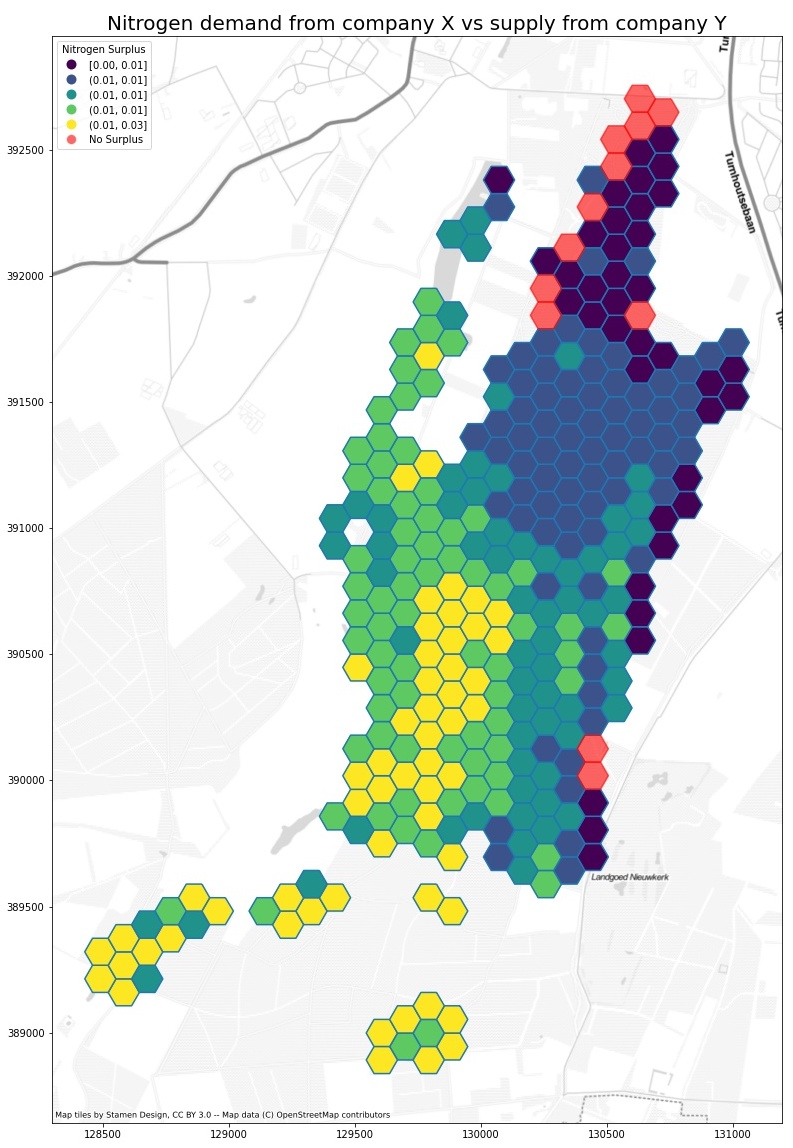
\includegraphics[width=\textwidth, height=\textheight, keepaspectratio]{Nitro.jpg}
    \caption{Nitrogen surplus visualized with LinearRings.}
    \label{fig:finalmap}
\end{figure}

\end{document}



